% !TeX root = ../main.tex
% Add the above to each chapter to make compiling the PDF easier in some editors.

\chapter{Stereo Rendering Optimization - Effort reduction}
The following chapter of optimization approaches targets the efficiency of rendering processes on the graphics chip itself. These approaches have little to no impact on CPU performance and tend to exploit and scale mostly with GPU power. 
Note again that only a subset of the listed methods was implemented due to time constraints. 

\section{Multiview stereo rendering} \label{MV_Stereo}
When rendering a stereo image using the naive method of simply going through the entire rendering pipeline once for each viewport, potentially a lot of computation is done twice with little or no change in data or parameters. 
With the general graphics pipeline (\autoref{fig:Gfx_pipeline}) in mind, it is clear that for example the vertex stage will see very little change in output as geometry and index buffers are largely the same between multiple stereo viewport passes with only minor shifts in the view matrices. Similarly, the geometry stage is commonly not dependent on specific eye data and as such it would be a waste to process with the same data twice. Once the rasterizer stage of the pipeline is reached, the situation changes as stereo separation means the two images have notably different content and work from one can not realistically be recycled in the other. 

\begin{figure}[htb]
  \centering
  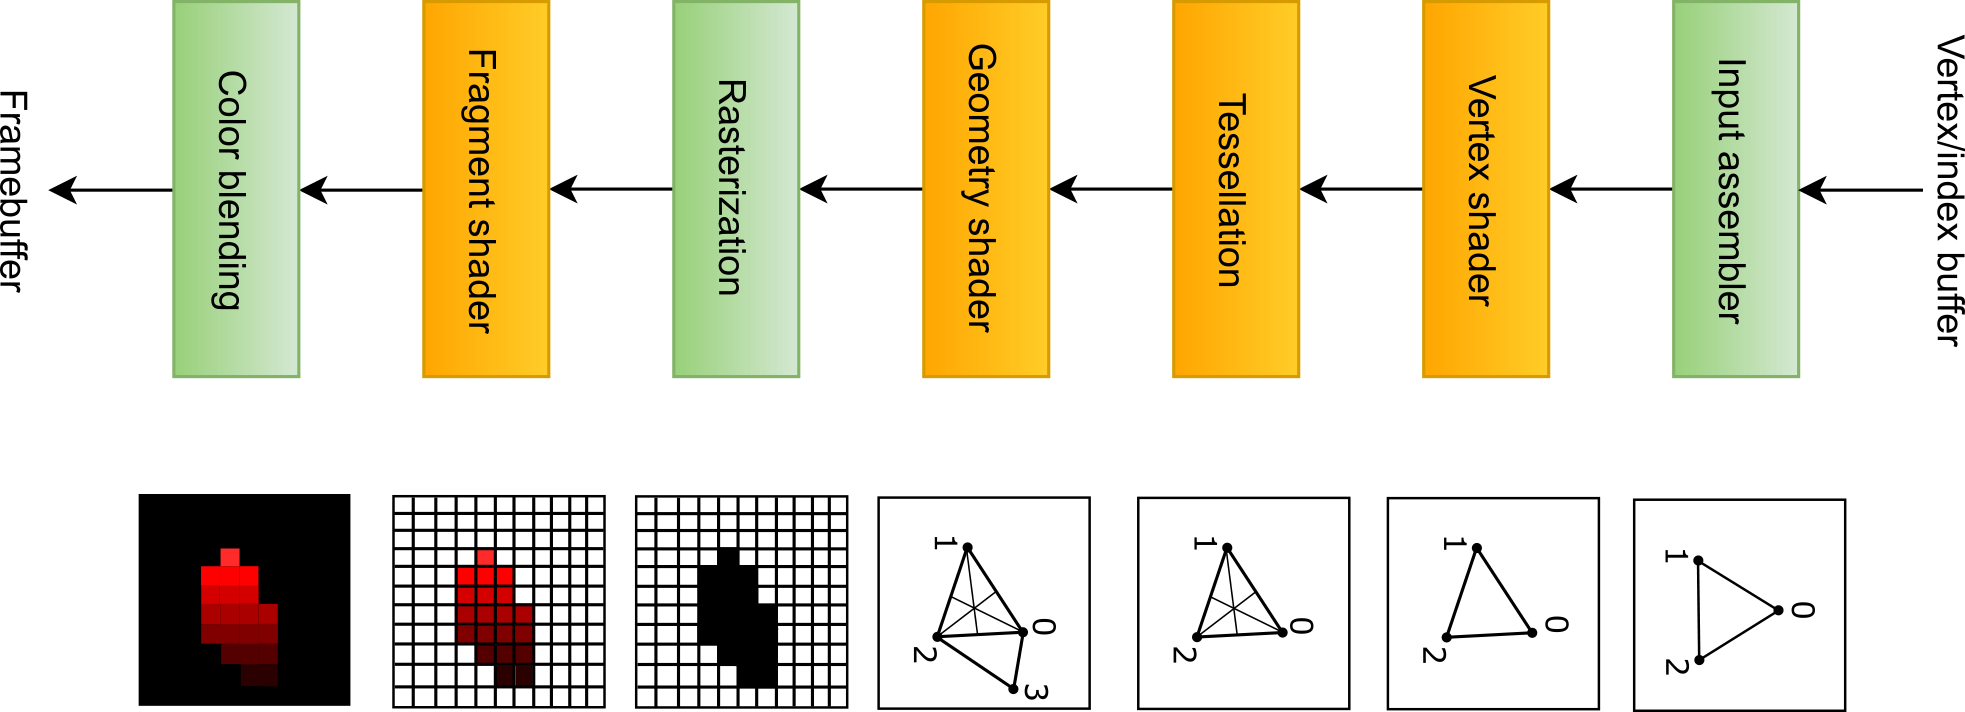
\includegraphics[width=0.8\textwidth]{pictures/vulkan_simplified_pipeline_L}
  \caption{Simplified graphics pipeline of a modern GPU (from \cite{Overvoorde.}, A. Overvoorde)} \label{fig:Gfx_pipeline}
\end{figure}

An optimization exploiting this is called multiview stereo rendering. It very quickly surfaced as an idea after the introduction of the Nvidia Geforce 8 and ATi Radeon HD 2000 series in 2006 and 2007 brought unified shader architectures to the mass market \cite{Lindholm.2008}\cite{Sommefeldt.2007}. Prior architectures relied on separate vertex and pixel shader units with relatively fixed capabilities and few ways to share data. Fully programmable shader units then allowed more customizable and efficient pipeline usage necessary for multiview to show any benefit. 
The lack of mainstream stereoscopic systems prohibited the feature from becoming more important until the official introduction of multiview extensions to graphics APIs like OpenGL (\codeword{GL_OVR_multiview}) and Vulkan (\codeword{VK_KHR_Multiview}, previously \codeword{_KHX} and \codeword{_NV}). 
The same resurgence saw the idea expanded and further optimized. In more recent vendor specific terms, Nvidia calls it Single Pass Stereo\cite{Cantlay.2016}, Simultaneous Multi-Projection\cite{Smith.2016} and Multi-View\cite{Bhonde.2018} rendering and AMD calls it LiquidVR multiview\cite{Gallagher.2016}\cite{Jez.2017}. The idea behind all these terms is the same, albeit with detail differences between the different flavors. \\

The core concept of multiview rendering is to submit all draw commands for a stereoscopic frame in one call instead of two separate passes, which can cut down CPU render and transfer time depending on the type and amount of data pushed to the GPU. Expensive synchronization barriers are essentially halved and all necessary writes are performed in a single go. This is illustrated - albeit strongly simplified - in \autoref{fig:MView_OnOff}, which makes it easily visible where multiview cuts out unnecessary work. 
As an addition, \textit{hardware} multiview rendering is to only perform those pipeline stages multiple times which actually produce notably different data for each eye, such as the rasterizer and pixel shader stages, while only running the earlier stages with little changes once. The data from stages run only once can then be reused by the multiply run stages with very little extra cost. This expanded technique improves pipeline efficiency and will scale heavily depending on workload. For fragment-heavy applications the benefit will be limited while high vertex or geometry loads tend to scale more optimally. Hardware acceleration requires additional registers and pipeline shortcuts in the chip itself, which constrains it to more modern GPU architectures built with it already in mind. Nvidia can be considered the main drivers behind this, having pushed the technology from parallel geometry projection in Maxwell's Multi-Projection Acceleration to Pascal's SMP adding lens-matched shading to better approximate the lens shape. Finally, to Turing's Multi-View with a doubling of available views and positional independence to support state of the art HMDs with canted displays \cite{Bhonde.2018}. \\
The small tradeoff is all relevant view data for each viewport having to be handed to the pipeline at once, creating a little higher memory overhead. Additionally, certain buffers such as geometry and indices for the vertex stage need to be uniform across all viewports and can not be altered for each eye as they are processed in a single pass. 

\begin{figure}[!ht]
\centering
     \subfloat[Simple stereo rendering loop flow\label{fig:MView_Off}]{%
       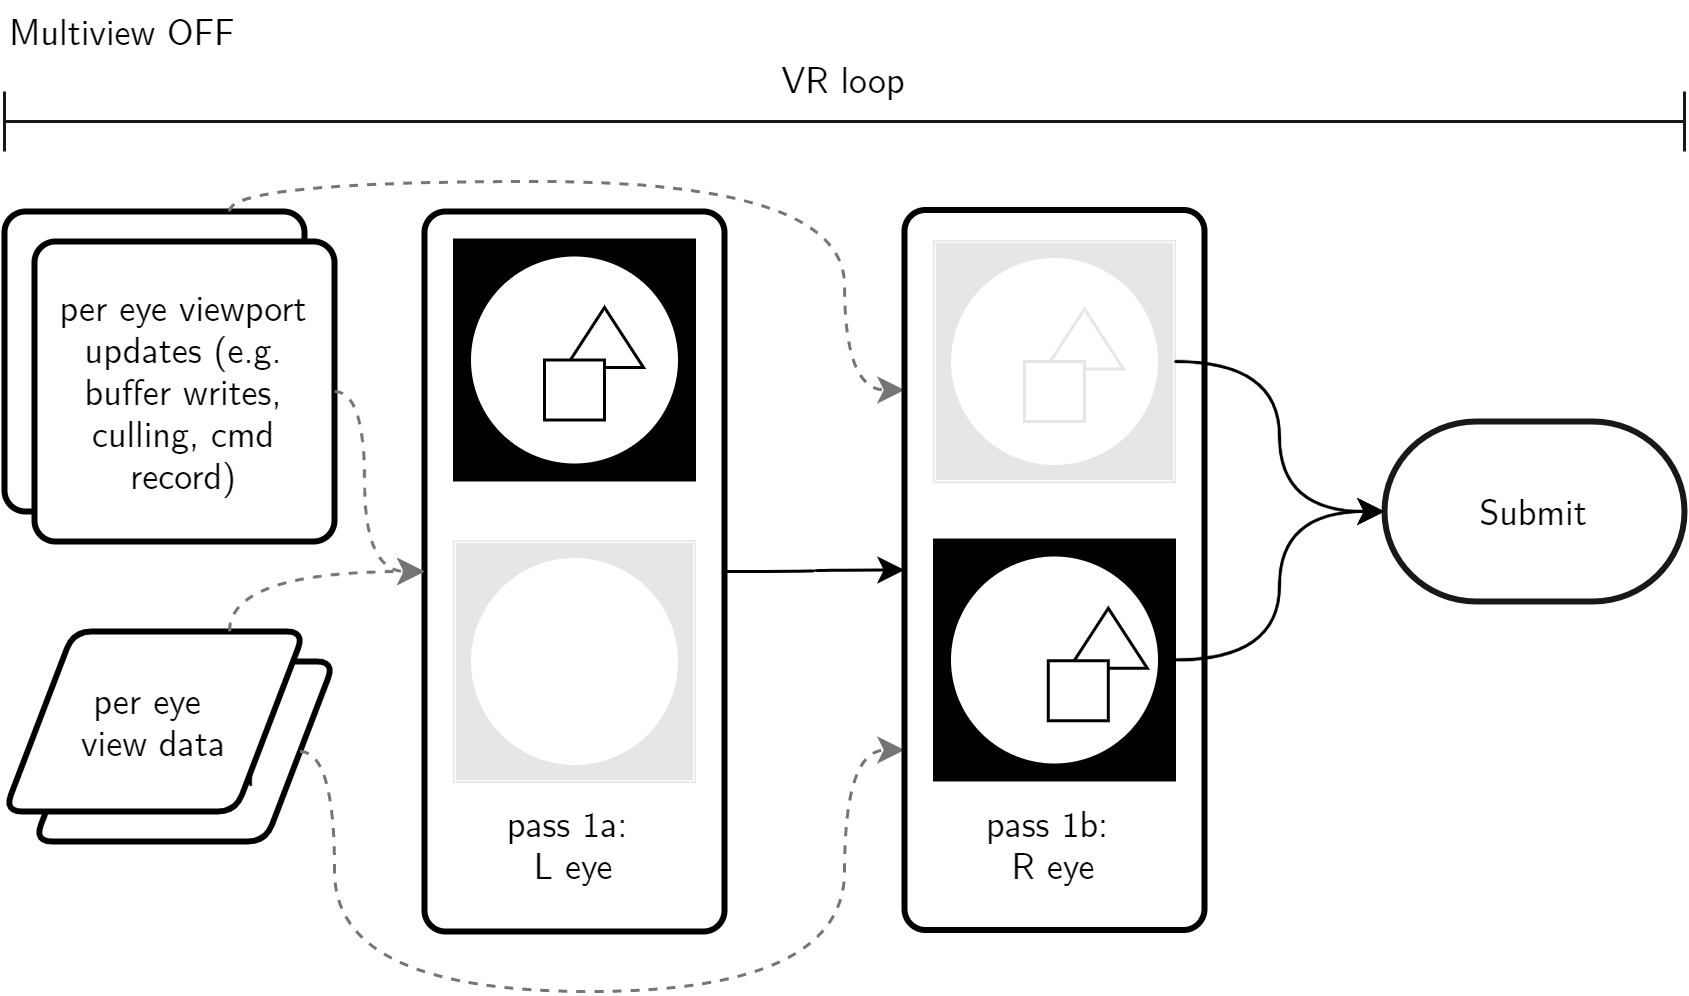
\includegraphics[height=8cm]{pictures/MView_Off}
     }
     \hfill
     \subfloat[Multiview stereo rendering loop flow\label{fig:MView_On}]{%
       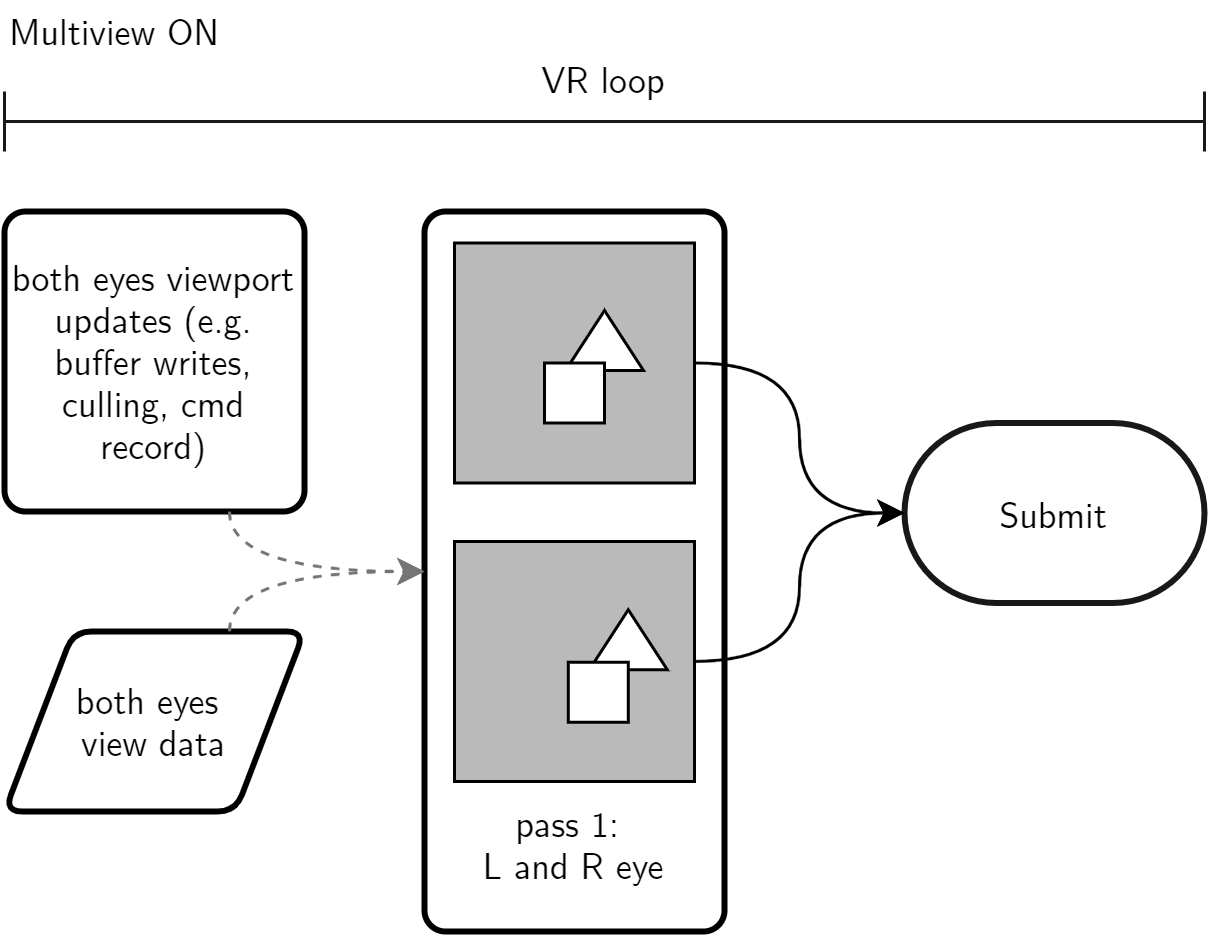
\includegraphics[height=8cm]{pictures/MView_On}
     }
     \caption{Simplified flow of standard stereo versus multiview render loops}
     \label{fig:MView_OnOff}
\end{figure}

Going by the user-maintained Vulkan Hardware Database \cite{Willems.2020}, the major GPU vendors offer multiview support in their architectures as follows: 
\begin{itemize}
\item Nvidia: hardware multiview from the Pascal generation and newer, software support from Kepler onward
\item AMD: software support from Graphics Core Next 1.0 onward \textcolor{red}{[TODO: hw support?]}
\item Intel: software support begins with Generation 9.0 (Skylake/Apollo Lake GT) onward under Windows, Generation 7.0 (Ivy Bridge GT) onward under Linux \textcolor{red}{[TODO: hw support?]}
\item Qualcomm: software support from Adreno 500 onward
\item ARM: software support from Bifrost onward, limited support on Midgard
\item Imagination: software support from Rogue onward
\end{itemize}
Note here, while support of the desktop parts is solid and stable, the ARM-based mobile chipsets often have incomplete or unstable drivers \cite{Willems.2019}\cite{JMC47.2018}. \\
For all submitted devices (892 at the time of writing) the database shows support coverage of 54\% on Windows systems, 69\% on Linux systems and only 23\% on Android. This statistic is not very reliable, since an undetermined portion of the submissions contains incomplete or flawed information such as drivers versioned as 0.0.0 or API versions reported as 0.0.1. 

\subsection{Estimated impact}
Impact of this extension is highly dependent on the specific workload, the used graphics hardware and the renderer structure. \\
Independent benchmark numbers are rare to find. In benchmarking the online racing simulation iRacing, Wolfgang Andermahr of ComputerBase GmbH attests a performance increase of between 14-21\% when testing on a Nvidia GTX 1060 and GTX 1080 at 5760 by 1080 pixels. While this is not a VR application, it gives a first impression of potential gains when rendering multiple viewports using hardware-accelerated multiview as is the case on these Pascal-based GPUs \cite{Andermahr.2016}.
Similarly, Croteam's Karlo Jez shows significant CPU performance gains for software multiview using AMD's LiquidVR suite, reducing CPU frame time in Serious Sam \gls{VR} from 9ms down to 7ms \cite{Jez.2017}. He specifically notes that this includes all stages of CPU rendering, even ones that are not connected to multiview, and adds that render command processing itself is halved from 4ms to 2ms by using software multiview. 
Going further from traditional desktop rendering, Mozilla Corp. reports performance improvement of up to 40\% when using the multiview extension for WebGL in a CPU-bound test application \cite{Serrano.2019}. 

Overall this gives inconsistent performance expectations, but it does provide a trend. It stands to reason that with rising CPU load and increasing number of virtual viewports, multiview rendering offers significant performance improvement in the double digit range. 

\subsection{Implementation specifics}
In Vulkan specifically, multiview is enabled through the \codeword{VK_KHR_multiview} extension. This extension's availability on the target hardware can be queried and if available, the individual hardware-dependent implementation is abstracted by Vulkan. \\
In the \gls{Tachyon} implementation of multiview, the following changes to the render loop are introduced: 
\begin{itemize}
\item The \gls{VR} render target adds \codeword{VK_KHR_GET_PHYSICAL_DEVICE_PROPERTIES_2} to the required instance extensions and \codeword{VK_KHR_MULTIVIEW} to the required device extensions during Vulkan instance and device creation at startup
\item the previously separate per-eye \gls{VR} render passes are merged into a single render pass
\item this \gls{VR} render pass incorporates the multiview pNext extension using a view mask and correlation mask of 0x11, with each of those bits representing one of the eyes
\item the Frustum Culling pass combines the two frustum checks with an early accept and outputs a merged set of draw call information
\item the second command buffer recording - previously intended for the second eye - in \codeword{OpenVR::RecordCommandBuffers()} is cut out as multiview render passes can only take a single unified set of command buffers
\item the underlying GLSL shader is modified to pick camera parameters based not only on a given camera index, but also the implicit \codeword{gl_viewIndex} as Vulkan multiview uses this integer to index the current viewport
\end{itemize}
The \gls{VR} render target's framebuffer, color attachment and depth attachment are already set up as dual-layered buffers which makes them readily compatible with multiview render passes. With these changes, the \gls{Tachyon} renderer is fully switched over to single pass stereo rendering. 